\section{Wellenleiter}
\subsection{Koaxial Leiter}
\subsubsection{Wellenwiderstand}

\begin{center}
    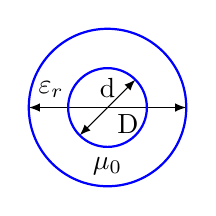
\begin{tikzpicture}
        \draw[latex-latex](-1,0)node[above right]{$\varepsilon_r$}--(1,0);
        \node[below right, yshift=1pt]{D};
        \draw[latex-latex, rotate=45](-0.5,0)--(.5,0);
        \node at (0,0)[above]{d};
        \draw[-, thick, blue](0,0) circle (1);
        \node at(0,-.75)[]{$\mu_0$};
        \draw[-, thick, blue](0,0) circle (0.5) ;
    \end{tikzpicture}


    D = Außendurchmesser

    d = Innendurchmesser
\end{center}
\vspace{-1em}

\begin{align*}
    Z_L = \frac{Z_{F0}}{2\pi}\sqrt{\frac{\mu_r}{\varepsilon_r}}\ln\left( \frac{r_a}{r_i} \right)  =\frac{60\Omega}{\sqrt{\varepsilon_r}}\cdot \ln{\frac{r_a}{r_i}}
\end{align*}

\subsubsection{Dämpfung}
Hin- und Rückleiter!\\
\underline{\textbf{Ohmsche Verluste}} $R\ll\omega L$
\[
    \alpha_L = \frac{\sqrt{\dfrac{f\cdot\mu}{\pi\cdot\sigma}}}{120\Omega}\cdot\frac{\sqrt{\varepsilon_r}}{D}\cdot\dfrac{1+\dfrac{D}{d}}{\ln \dfrac{D}{d}}
\]

Dämpfungsminimum für $ \frac{1+\tfrac{D}{d}}{\ln \tfrac{D}{d}} = 1 $\\ bei vorgegebenen Außendurchmesser: $ \frac{D}{d} =3,59 $\\

\underline{\textbf{Dielektrische Verluste}} $G\ll\omega C$,$\tan\delta= (^G/_{\omega C})$
\[
    \alpha_d = \frac{\sqrt{\varepsilon_r}\pi f}{c_0}\cdot\tan\delta \sim f
\]

\subsection{Mikrostreifenleiter}
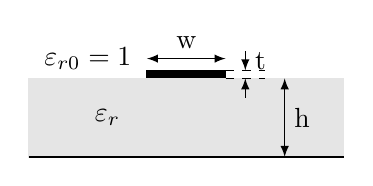
\begin{tikzpicture}
    %Leiterbahn
    \filldraw[black]    (1,1)   rectangle (2,1.1);
    %Dielektrika
    \filldraw[black!10] (-.5,0) rectangle (3.5,1);
    \draw[-,thick](-.5,0)--(3.5,0);
    %Bemassungen
    \draw[latex-latex](2.75,0)--(2.75,1) node[midway, right]{h};
    \draw[latex-latex](1,1.25)--(2,1.25) node[midway, above]{w};
    \draw[dashed](2,1)      --(2.5,1);
    \draw[dashed](2,1.1)    --(2.5,1.1);
    \draw[latex-](2.25,1)   --(2.25,.75);
    \draw[latex-](2.25,1.1) --(2.25,1.35) node[midway, right]{t};
    %Dielektrizitätskonstanten
    \node at (.5,.5)[]{$\varepsilon_r$};
    \node at (.25,1.25)[]{$\varepsilon_{r0}=1$};
\end{tikzpicture}

\subsubsection{Effektive Permittivitätszahl}
Unterschiedliche Phasengeschwindigkeit $\rightarrow$ Dispersion
\[
         \varepsilon_{r,\texttt{eff}}  = \frac{\varepsilon_r+1}{2}+\frac{\varepsilon_r-1}{2\sqrt{1+10\cdot\frac{\text{h}}{\text{w}}}} \\
\]

Je größer $\dfrac{\mathrm{w}}{\mathrm{h}}$ desto mehr nähert sich $\varepsilon_{r,\texttt{eff}}$ an $\varepsilon_r$ und 
\[
    \lambda = \frac{\lambda_0}{\sqrt{\varepsilon_{r,\texttt{eff}}\cdot\mu_{r,\texttt{eff}}}}
\]

\subsubsection[Schmale Streifen]{Schmale Streifen (ca 20-200$\Omega$)}
\[
    Z_L = \frac{60\Omega}{\sqrt{\varepsilon_{r,\texttt{eff}}}}\cdot\ln\left(\frac{8\mathrm{h}}{\mathrm{w}}+\frac{\mathrm{w}}{4\mathrm{h}}\right)
\]
\subsubsection[Breite Streifen]{Breite Streifen (ca 20-200$\Omega$)}
\[
    Z_L = \frac{120\pi\Omega}{\sqrt{\varepsilon_{r,\texttt{eff}}}}\cdot\frac{1}{\dfrac{\mathrm{w}}{\mathrm{h}}+2,42-0,44\cdot\dfrac{\mathrm{h}}{\mathrm{w}}+\left(1-\dfrac{\mathrm{h}}{\mathrm{w}}\right)^6}
\]

\subsection{Hohlleiter}
\[
    f_c = \frac{c_0}{2a}
\]

\subsection{VSWR (Voltage Standing Wave Ratio) und Return Loss}\label{sec:VSWR}
\underline{VSWR}
\begin{align*}
    s   & = \mathrm{VSWR} = \frac{1+|r|}{1-|r|}\geq 1 \\
    |r| & = \frac{s-1}{s+1}
\end{align*}
\underline{Return Loss}
\[
    \alpha_r = -20\log(r)dB
\]
\underline{Missmatch Loss}
\[
    \mathrm{ML} = -10\log(1-r^2)dB
\]
\subsection{Lichtwellenleiter oder Glasfaser}

\begin{description}
    \setlength\itemsep{1pt}
    \item APF := All Plastic Fiber
    \item POF := Polymerfaser
    \item LWL := Lichtwellenleiter
    \item $B\cdot l$ := Bandbreitenlängenprodukt
\end{description}

\begin{description}
    \item \underline{Dispersion:}

          {\small Die von der Frequenz des Lichts abhängende
              Ausbreitungsgeschwindigkeit des Lichts in Medien. Dies hat zur Folge,
              dass Licht an Übergangsflächen unterschiedlich stark gebrochen wird.
              Somit verflacht sich beispielsweise ein (Dirac-)Impuls zu einer Gauß'schen
              Glocke.
          }
    \item \underline{Stufenprofil:}

          {\small Multimode: leichtes Einkoppeln, geringes $B\cdot l$ wegen
              Modendispersion

              Single/Monomode: schwieriges Einkoppeln, großes $B\cdot l$, keine
              Modendispersion
          }
    \item \underline{Gradientenprofil:}

          {\small Multimode: Kompromiss beim Einkoppeln und Reichweite mit $B\cdot l$}
    \item \underline{Bandbreitenlängenprodukt:}

          {\small $B' =  B\cdot l[\frac{MHz}{km}]$ = konstant

              $B \sim \frac{1}{l}$ und $l\sim \frac{1}{B}$

              Bandbreite ist gegen Übertragungslänge austauschbar, solange
              Dämpfung keine Rolle spielt.
          }
\end{description}
%\newpage
%\subsection{Leitungsparameter}
%\subsubsection{Streifenleitung / Parallele Platten}
%Für Sinus-Anregung:
%\begin{align*}
%	I(l) & = \frac{U}{Z_L} = \underbrace{\frac{U_0}{Z_L}}_{I_0}\cdot e^{-j\beta l\cdot e^{j\omega t}}                         \\
%	U(l) & = \int \vec{E} d\vec{s} \stackrel{b\gg d}{=} E\cdot d \rightarrow  &E = \frac{U_0}{d}\cdot^{-j\beta l}\cdot\vec{e}_x \\
%	I(l) & = \oint \vec{H} d\vec{s} =  H\cdot b \rightarrow &H = \frac{I_0}{b}\cdot^{-j\beta l}\cdot\vec{e}_y                  % \\
%	% \vec{E}(r, z) & = \frac{I}{2\pi r}\cdot Z_F\cdot e^{-j\beta z} \cdot\vec{e}_r                                                      \\
%	%               & = \frac{\hat{U}}{r \cdot\ln{(^{2b}/_{2a})}}\cdot e^{-j\beta z}\cdot\vec{e}_r
%\end{align*}
%$ \mathbf{b} $: Platten\textbf{breite} \qquad $ \mathbf{d} $: Abstand zwischen den Platten\\
%
%\begin{minipage}[t]{0.4\columnwidth}
%\begin{tikzpicture}
    \tikzset{cross/.style={cross out, draw=black, minimum size=2*(#1-\pgflinewidth), inner sep=0pt, outer sep=0pt},
        %     %default radius will be 1pt. 
        cross/.default={3.5pt}}

        %Untereplatte
        \draw[-](0,0)--(0,0.35);
        \draw[-](2,0)--(2,0.35);

        \draw[-](0,0)--(2,0);
        \draw[-](0,0.35)--(2,0.35);

        \draw[-](0,0.35)--(0.3,0.65);
        \draw[-](2,0)--(3,1);
        \draw[-](2,0.35)--(3,1.35);

        \draw[-](1,0.175) circle (0.15);
        \draw[-,fill=black!100] (1,0.175) circle (0.05);

        %Obere Platte
        \draw[-](0,0.65)--(0,1);
        \draw[-](2,0.65)--(2,1);

        \draw[-](0,0.65)--(2,0.65);
        \draw[-](0,1)--(2,1);

        \draw[-](0,1)--(1,2);
        \draw[-](2,1)--(3,2);
        \draw[-](2,0.65)--(3,1.65);

        \draw[-](1,0.825) circle (0.15);
        \draw(1,0.825) node [cross] {};
   
\end{tikzpicture}

%\end{minipage}
%\begin{minipage}[b][1cm]{0.6\columnwidth}
%	\begin{flalign*}
%		&R'=\frac{2}{\delta\kappa b}\left[ \frac{\Omega}{m} \right] & &L'=\frac{\mu d}{b} \left[\frac{H}{m}\right]&\\
%		&G'=\frac{\kappa b}{d} \left[ \frac{S}{m} \right] &
%		&C'=\frac{b\varepsilon}{d} \left[\frac{F}{m}\right]
%	\end{flalign*}
%\end{minipage}
%%
%%
%%{\renewcommand*{\arraystretch}{0.2}
%%	\begin{tabularx}{0.5\columnwidth}{X}
%%		\hline
%%		\[R'=\frac{2}{\delta\kappa b}\] \\
%%		\hline
%%		\[L'=\frac{\mu d}{b}\]         \\
%%		\hline
%%		\[G'=\frac{\sigma b}{d}\]      \\
%%		\hline
%%		\[C'=\frac{b\varepsilon}{d}\]  \\
%%		\hline
%%	\end{tabularx}
%%}
%
%\subsubsection{Doppelleitung}
%$ \kappa $: Leitwert des Dielektrikums \qquad $ \kappa_L $ Leitwert des Leiters\\
%$ \mathbf{r} $: Leiterradius \qquad $ \mathbf{d} $: Abstand zw. Leitermitten
%
%\begin{minipage}[t]{0.4\columnwidth}
%	\begin{tikzpicture}
    \tikzset{cross/.style={cross out, draw=black, minimum size=2*(#1-\pgflinewidth), inner sep=0pt, outer sep=0pt},
        %     %default radius will be 1pt. 
        cross/.default={3.5pt}}

        %linker Außenleiter
        \draw[-](-0.53,0.53)--(0.97,2.03);

        
        \draw[-](48:0.75) arc (48:312:0.75);

        %linker Innenleiter
        \draw[dashed](-0.106,0.106)--(0.41,0.622);
        \draw[dashed](0.106,-0.106)--(0.922,0.71);

        \draw[-](0,0) circle (0.15);
        \draw(0,0) node [cross] {};


        
        %%%%%%%%%%%%%%%%%%%%%%%%%%%%%%%%%%%%%%%%%%%%%%%%%%%%%%%%%%%
        %%%%%%%%%%%%%%%%%%%%%%%%%%%%%%%%%%%%%%%%%%%%%%%%%%%%%%%%%%%

        %Rechter Außenleiter
        \draw[-](0.48,0.58)--(1.97,2.03);
        \draw[-](1.53,-0.53)--(2.13,0.07);
        \draw([shift={(228:0.75)}]1,0) arc (-132:132:0.75);

        %Rechter Innenleiter
        \draw[dashed](0.894,0.106)--(1.41,0.622);
        \draw[dashed](1.106,-0.106)--(1.622,0.41);

        \draw[-](1,0) circle (0.15);
        \draw[-,fill=black!100] (1,0) circle (0.05);

        

\end{tikzpicture}

%\end{minipage}
%\begin{minipage}[b][4cm]{0.6\columnwidth}
%	\begin{flalign*}
%		&R'=\frac{1}{\pi a\delta\kappa_L} \left[ \frac{\Omega}{m} \right] &\\
%		&L'= \frac{\mu}{\pi} \cosh^{-1}\frac{d}{2r} \left[\frac{H}{m}\right]&\\
%		&G'= \frac{\pi\kappa}{\cosh^{-1}(^d/_{2r})} \left[ \frac{S}{m} \right] &\\
%		&C'=\frac{\pi\varepsilon}{\cosh^{-1}(^d/_{2r})} \left[\frac{F}{m}\right]
%	\end{flalign*}
%\end{minipage}
%
%%{\small\[
%%	\text{cosh am TR: MENU $\rightarrow$ 1; OPTN $\rightarrow$ 1 $\rightarrow$ 5}\\
%%	\]}
%%\begin{tikzpicture}
    \tikzset{cross/.style={cross out, draw=black, minimum size=2*(#1-\pgflinewidth), inner sep=0pt, outer sep=0pt},
        %     %default radius will be 1pt. 
        cross/.default={3.5pt}}

        %linker Außenleiter
        \draw[-](-0.53,0.53)--(0.97,2.03);

        
        \draw[-](48:0.75) arc (48:312:0.75);

        %linker Innenleiter
        \draw[dashed](-0.106,0.106)--(0.41,0.622);
        \draw[dashed](0.106,-0.106)--(0.922,0.71);

        \draw[-](0,0) circle (0.15);
        \draw(0,0) node [cross] {};


        
        %%%%%%%%%%%%%%%%%%%%%%%%%%%%%%%%%%%%%%%%%%%%%%%%%%%%%%%%%%%
        %%%%%%%%%%%%%%%%%%%%%%%%%%%%%%%%%%%%%%%%%%%%%%%%%%%%%%%%%%%

        %Rechter Außenleiter
        \draw[-](0.48,0.58)--(1.97,2.03);
        \draw[-](1.53,-0.53)--(2.13,0.07);
        \draw([shift={(228:0.75)}]1,0) arc (-132:132:0.75);

        %Rechter Innenleiter
        \draw[dashed](0.894,0.106)--(1.41,0.622);
        \draw[dashed](1.106,-0.106)--(1.622,0.41);

        \draw[-](1,0) circle (0.15);
        \draw[-,fill=black!100] (1,0) circle (0.05);

        

\end{tikzpicture}

%%{\renewcommand*{\arraystretch}{0.2}
%%	\begin{tabularx}{0.5\columnwidth}{|X|}
%%		\hline
%%		\[R  = \frac{1}{\pi a\delta\sigma_c}\]              \\
%%		\hline
%%		\[L = \frac{\mu}{\pi} \cosh^{-1}\frac{d}{2a}\]      \\
%%		\hline
%%		\[G = \frac{\pi\sigma}{\cosh^{-1}(^d/_{2a})}\]      \\
%%		\hline
%%		\[C = \frac{\pi\varepsilon}{\cosh^{-1}(^d/_{2a})}\] \\
%%		\hline
%%\end{tabularx}}
%
%\subsubsection{Koaxialleitung}
%%{\small\[
%%	a = \text{innen Radius} \qquad b = \text{außen Radius} \\
%%	\]}
%$ r_i $: Innenradius \quad $ r_a $: Außenradius
%\begin{align*}
%	\vec{H}(r, z)         & = \frac{\hat{I}}{2\pi r}\cdot e^{-j\beta z}\cdot\vec{e}_\varphi                   \\
%	\vec{E}(r, z)         & = \frac{\hat{I}}{2\pi r}\cdot Z_{F0}\cdot e^{-j\beta z} \cdot\vec{e}_r
%	& = \frac{\hat{U}}{r \cdot\ln{(^{r_a}/_{r_i})}}\cdot e^{-j\beta z}\cdot\vec{e}_r        \\
%	S_{av} & = \frac{1}{2}\cdot\left( \frac{\hat{I}}{2\pi r}\right)^2\cdot Z_{F0}
%\end{align*}
%\begin{minipage}[c][2cm]{0.4\columnwidth}
%%	\begin{tikzpicture}
    \tikzset{cross/.style={cross out, draw=black, minimum size=2*(#1-\pgflinewidth), inner sep=0pt, outer sep=0pt},
        %     %default radius will be 1pt. 
        cross/.default={3.5pt}}

        %Außenleiter
        \draw[-](-0.53,0.53)--(1.07,2.13);
        \draw[-](0.53,-0.53)--(2.23,1.17);

        \draw[-](0,0) circle (0.75);

        %Innenleiter
        \draw[-](-0.106,0.106)--(0.41,0.622);
        \draw[-](0.106,-0.106)--(0.622,0.41);

        \draw[-](0,0) circle (0.15);
        \draw(0,0) node [cross] {};

\end{tikzpicture}

%	\begin{center}
    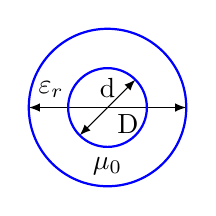
\begin{tikzpicture}
        \draw[latex-latex](-1,0)node[above right]{$\varepsilon_r$}--(1,0);
        \node[below right, yshift=1pt]{D};
        \draw[latex-latex, rotate=45](-0.5,0)--(.5,0);
        \node at (0,0)[above]{d};
        \draw[-, thick, blue](0,0) circle (1);
        \node at(0,-.75)[]{$\mu_0$};
        \draw[-, thick, blue](0,0) circle (0.5) ;
    \end{tikzpicture}


    D = Außendurchmesser

    d = Innendurchmesser
\end{center}
\vspace{-1em}

%\end{minipage}
%\begin{minipage}[c][4cm]{0.6\columnwidth}
%	\begin{flalign*}
%		&R'=\frac{1}{2\pi\delta\kappa_L}\left(\frac{1}{r_a}+\frac{1}{r_i}\right) \left[ \frac{\Omega}{m} \right] &\\
%		&L'=\frac{\mu_0\mu_r}{2\pi}\ln\frac{r_a}{r_i} \left[\frac{H}{m}\right]&\\
%		&G'=\frac{2\pi\kappa}{\ln(r_a/r_i)} \left[ \frac{S}{m} \right] &\\
%		&C'=\frac{2\pi\varepsilon_0 \varepsilon_r}{\ln(r_a/r_i)} \left[\frac{F}{m}\right]
%	\end{flalign*}
%\end{minipage}
%%
%%
%%{\renewcommand*{\arraystretch}{0.2}
%%	\begin{tabularx}{0.5\columnwidth}{|X|}
%%		\hline
%%		\[R=\frac{1}{2\pi\delta\sigma_c}\left[\frac{1}{a}+\frac{1}{b}\right]\] \\
%%		\hline
%%		\[L=\frac{\mu}{2\pi}\ln\frac{b}{a}\]                                   \\
%%		\hline
%%		\[G=\frac{2\pi\sigma}{\ln(^b/_a)}\]                                    \\
%%		\hline
%%		\[C=\frac{2\pi\varepsilon}{\ln(^b/_a)}\]                               \\
%%		\hline
%%\end{tabularx}}
%\vspace{1ex}
%\subsubsection{Allgemein}
%Für beliebige Leitergeometrie gelten folgende Zusammenhänge:
%\[
%LC = \mu\varepsilon \quad \text{und} \quad \frac{G}{C} = \frac{\sigma}{\varepsilon}
%\]
%Innere Induktivität:
%\[
%L_i = \frac{R}{w}
%\]
%\textbf{\color{red}{Leitungen gehen HIN und ZURÜCK!!!}\\
%	\color{red}{Länge verdoppeln!!!}
%}